\documentclass[a4paper,12pt]{book}
\usepackage[utf8]{inputenc}
\usepackage{graphicx}
\usepackage{amsmath}
\usepackage{algpseudocode}
\usepackage{amsmath, amssymb}

\DeclareMathOperator{\EX}{\mathbb{E}}% expected value
\DeclareMathOperator*{\argmax}{arg\,max}
\DeclareMathOperator*{\argmin}{arg\,min}

\begin{document}

\author{Willem}
\title{Notes while reading Reinforcement learning an introduction (Sutton/Barto)}
\date{January 2013}

\frontmatter
\maketitle
\tableofcontents

\mainmatter
\chapter{Introduction}
\chapter{Mutli-armed bandits}
\chapter{Finite Markov Decision Process}

\section{Summary}

MDP's are a formal framework to model sequential decision making. It can handle immediate and delayed rewards, incorporating state.

\subsection{Agent-Environment Interface}

\begin{enumerate}
	\item agent: Leaner and decision maker.
	\item environment: The thing the agent interacts with.
	\item $P(s', r|s,a)$: dynamics of the system (as probability distribution) 
\end{enumerate}

If the next state $S_{t+1}$ only depends on the current state $S_t$ and the input $A_t$, then the state is said to have the \textbf{Markov property} .

\begin{figure}[H]
	\centering
	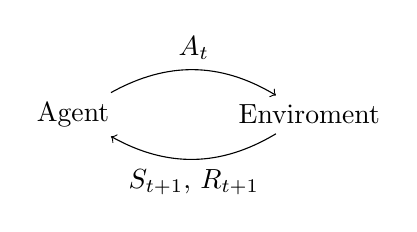
\begin{tikzpicture}
	
	\node at (1, 0) (a) {Agent};
	\node at (4, 0) (b) {Enviroment};
	
	\draw [->, auto, bend left] (a) to node {$A_t$} (b);
	\draw [->, auto, bend left] (b) to node {$S_{t+1}$, $R_{t+1}$} (a);
	\end{tikzpicture}
	\caption{Agent Environment}
	\label{fig:agent-enviroment}
\end{figure}

\subsection{Goals and rewards}

The \textbf{reward hypothesis} say's that all goals/purposes can be expressed as maximizing reward.

Reward should only communicate \textbf{what} needs to be done, not \textbf{how}.

\subsection{Returns and episodes}
An \textbf{episodial task} has a finite number of steps, until it stops in the absorbing state. $G_t = R_{t+1} + R_{t+2} + ... + R_{T}$.

A \textbf{continuing task} never stops, so it keeps getting rewards. So an extra concept \textbf{discount factor}($\gamma$) is needed to define the expected reward.  

\begin{equation}
\begin{split}
G_T & = R_{t+1} + \gamma R_{t+2} + ... \\
& = \sum_{k=0}^{\infty}\gamma R_{t+k+1} \\
& 0 \leq \gamma \leq 1
\end{split}
\label{eq:expected return continuing task}
\end{equation}

The discount factor is a geometric series, and equals to one.
\begin{equation}
\sum_{k=0}^{\infty} \gamma ^k = \frac{1}{1-\gamma}
\label{eq:discount factor geometry series}
\end{equation}

\subsection{Policies and value function}
The \textbf{state-value function} expressed how it is to be in a certain state under a certain policy($\pi$). It has a recursive definition that is derived in equation~\ref{eq:bellman equation value function derivation} and known as the \textbf{bellman equation}.

\begin{equation}
\begin{split}
V_{\pi}(s) & = \EX\left[G_t | S_t = s\right]\\
& = \EX\left[\sum_{k=0}^\infty \gamma^k R_{t + k + 1} | S_t = s\right]\\
& = \EX\left[R_{t+1} + \gamma G_{t+1} | S_t = s \right]\\
& = \sum_a \pi(a|s)\sum_{s',r} p(s', r|s,a)( r + \gamma \EX_\pi[G_{t+1}|S_{t+1}=s']) \\
& = \sum_a \pi(a|s)\sum_{s',r} p(s', r|s,a)( r + \gamma v_\pi(s'))
\end{split}
\label{eq:bellman equation value function derivation}
\end{equation}

The value of taking action $a$ under state $s$ is defined by the \textbf{action-value function} equation~\ref{eq:action-value function}.

\begin{equation}
\begin{split}
q_\pi(a, s) 
& = \EX[G_t | S_t = s, A_t = a]\\
& = \EX\left[\sum_{k=0}^\infty \gamma^k R_{t + k + 1} | S_t = s, A_t = a\right]\\
& = \sum_{r,s'} p(s', r|s,a)( r + \gamma v_\pi(s'))
\label{eq:action-value function}
\end{split}
\end{equation}

\subsection{Optimal policies and optimal value function}
Solving a \textbf{reinforcement learning} problem is finding a policy that gets a lot of reward. The best possible policy is called the \textbf{optimal policy}, the value-state function of this policy is the \textbf{optimal state-value function} $v_*(s)=\max_{\pi}v_\pi(s)$. And the action-value function is the \textbf{optimal value-state function} $q_*(s, a)= \max_{\pi} q_\pi (s, a)$ 

\begin{equation}
\begin{split}
v_* 
& = \max_a q_\pi (s, a) \\
& = \max_a \EX\left[ G_t | S_t=a, A_t=a \right] \\
& = \max_a \EX\left[ R_{t+1} + \gamma G_t | S_t=a, A_t=a \right] \\
& = \max_a \EX\left[ R_{t+1} + \gamma V_*(S_{t+1}) | S_t=a, A_t=a \right] \\
& = \max_a \sum_{s}p(s', r | a, s) [r+ \gamma V_*(s')] \\
\end{split}
\label{eq:bellman optimality equation state-value function derivation}
\end{equation}

The optimal state-value and action-value functions lead to \textbf{the bellman optimality equations} equation~\ref{eq:bellman optimality equation state-value function derivation} and equation~\ref{eq:bellman optimality equation action-value function derivation}

\begin{equation}
\begin{split}
q_*(s, a) 
& = \EX\left[ R_{t+1} + \gamma \max_{a'} q(S_{t+1},a') | S_t=s, A_t=a \right] \\
& = p(s' r | s, a)[ r + \gamma \max_{a'} q(s', a)]
\end{split}
\label{eq:bellman optimality equation action-value function derivation}
\end{equation}

\section{Exercises}

\subsection{Exercise 3.1}
A Robot in a maze has a delayed reward, and needs to make a sequence of decisions. The position of the robot in the maze is the state, and the input is the decisions left/right/straight ahead. The reward is -1 until the absorbing state, which has a reward of zero.

A automatic poker player can be a mdp, the state is the current cards in the hand and the table. 
\chapter{Dynamic Programming}
\section{Summary}
Dynamic programming is a \textbf{collection of algorithms} that can be used to find the \textbf{optimal policy}. It assumes a perfect model of the system (MDP) and uses a lot of computational power. 

\begin{equation}
v_*(s) = \max_a \sum_{s',r} p(s', r | s, a)[r + \gamma v_*(s')]
\label{eq:bellman optimality equation state-value function}
\end{equation}

\begin{equation}
q_*(s, a) = \sum_{s', r} p(s', r | s, a) [r + \gamma \max_{a'} q_*(s', a')]
\label{eq:bellman optimality equation action-value function}
\end{equation}

\subsection{Policy evaluation}
The bellman equation from \ref{eq:bellman equation value function derivation} can be converted into an iterative method called \textbf{iterative policy evaluation} to find the value function. It takes the expected value over all the same next states. All updates in dynamic programming are called \textbf{expected updates}, because they are based on expectation over all possible next states rather then the sample next states.

\begin{equation}
\begin{split}
v(s)_{k+1} 
& = \EX_\pi\left[ R_{t+!} + \gamma v_k(S_{k+1}) | S_t = s \right] \\
& = \sum_a \pi(a | s) \sum_{s', r} p(s', r | s, a) \left[r + \gamma v(s')\right] \\
\end{split}
\label{eq:iterative policy evaluation update rule}
\end{equation}

\subsection{Policy improvement}
\begin{equation}
\begin{split}
q_\pi(a, s) & = \EX\left[R_{t+1} + \gamma v_\pi(S_{t+1}) | S_t = s, A_t = a \right]\\
& = \sum_{s', r} p(s', r | s, a)\big[r + \gamma v_\pi(s')\big]
\end{split}
\label{eq:policy improvement, select the next action}
\end{equation}

Given a policy $\pi$ and value function $v_\pi(s)$, one action $a$ can be selected that maximizes equation~\ref{eq:policy improvement, select the next action} and all sequential actions follow the policy $\pi$. The \textbf{policy improvement theorem}  say's that if a new policy $\pi'$ satisfies equation~\ref{eq:policy improvement theorem condition}, the the new policy will satisfy equation~\ref{eq:policy improvement theorem result}. And be as good or better then the original policy.(proof on page 78-79 of the book)

\begin{equation}
q_\pi(s, \pi'(s)) \geq v_\pi(s)
\label{eq:policy improvement theorem condition}
\end{equation}

\begin{equation}
v_{\pi}(s) \leq v_{\pi'}(s)
\label{eq:policy improvement theorem result}
\end{equation}

The new improved policy $\pi'$ is formally written down in equation~\ref{eq:greedy policy action-value}. The corresponding value function is formally written down in equation~\ref{eq:greedy policy value function to bellman equation}. Where we \textbf{end up with the bellman optimality equation}. Indicating that the policy can improve until it's the optimal policy.

\begin{equation}
\begin{split}
\pi'(s) & = \argmax_a q_\pi (s, a) \\
& = \argmax_a \EX\left[ R_{t+1} + \gamma v_\pi(S_{t+1} | S_t = s, A_t = a) \right] \\
& = \argmax_a \sum_{s',r} p(s', r|s, a)\left[r + \gamma v_{\pi}(s')\right]
\end{split}
\label{eq:greedy policy action-value}
\end{equation}

\begin{equation}
\begin{split}
v_{\pi'}(s) 
& = \max_a \EX\left[ R_{t+1} + \gamma v_\pi'(S_{t+1}) | S_t = s, A_t=a \right] \\
& = \max_a \sum_{s', r}p(s', r|s, a)\left[r + \gamma v_{\pi'}(s')\right]
\end{split}
\label{eq:greedy policy value function to bellman equation}
\end{equation}

\subsection{Policy iteration}

The iterative process of evaluating a policy, and then creating a new policy that is greedy towards the old one is called \textbf{policy iteration}.

\subsection{Value iteration}

Instead of evaluating the complete policy first, and then improving the policy. The policy can be improved after every state evaluation. Effective \textbf{turning the bellman optimality equation into the iterative update} of equation~\ref{eq:value iteration}.

\begin{equation}
v_{k+1} = \max_a = \sum_{s',r} p(s', r| s, a)\big[ r + \gamma v_k(s')\big]
\label{eq:value iteration}
\end{equation}

\subsection{Generalized policy iteration}
The iterative process of repeatedly evaluating a policy and using it to create an improved version of that policy, is referred to as \textbf{generalized policy iteration} or short GPI. Both policy iteration and value iteration are GPI, as do many stochastic methods.


\section{Exercises}

\subsection{Exercise 4.8}
The reward is only obtained when the capital is above 99. When the capital is at 50, there is a 50\% chance you can win the game. So this obviously is the optimal policy. When you reach 51: it would be rather odd to bet the entire capital, as you don't need to risk it all to reach 100. Bigger downside, but same upside. So the best course of action is to bet with 1, see if you can grow this above 50. If you lose it, you still have a 50\% chance to win by betting it all.
\chapter{Monte Carlo Methods}

\section{Exercises}

\subsection{Exercise 5.1 page 94}
The last 2 rows in the rear means you either have 21, or 20, which means the odd's are very good you will win. (hence high value function)

The last row on the left means the dealer has an ace, so it's at an advantage to get a higher score.

The front row's are higher on the upper diagram, as there is a usuable ace. Which means that if you get a bad hit that put's you over 21. It can count as 1.

\subsection{Exercise 5.2 page 94}
As this is Markov process eg. The cards drawn are not exhaustible. The odds of winning on the second time your in the same state is just as good as the first time.

\subsection{Exercise 5.4 page 99}
The "Append G to Returns ($S_{t} , A_{t}$) would be replaced by increasing a count and added it as running average to some table.

\subsection{Exercise 5.5 page 105}
\textbf{question: Consider an MDP with a single Non-terminal state and a single action that transitions back to the nonterminal state with probability $p$ and transitions to the terminal state with probability $p-1$. Let the reward be != on all transitions, and let $\gamma = 1$. Suppose you observe one episode that lasts 10 steps, with a return of 10. What are the first-visit and every visit estimators of the value of the non-terminal state. }

10 Steps means 9 towards the non-terminal, and one towards the terminal. The rewards are all-way's the same so the final cost=10. 

If $\gamma = 1$ then $G=G+\gamma R_{k+1}$ in every iteration. 

In case of all visit the complete horizon counts 10 times in the non-terminal state, as the 10th time we leave the non-terminal state for good and enter the terminal state. $(1+2+3+4+5+6+7+8+9+10)/10 = 55/10 = 5.5$ So the value is 5.

In case of the first-visit, we only count the first visit which has a reward of 1.

\subsection{Exercise 5.6 page 108}
\textbf{question: What is the equation analogous to (5.6) for action values $Q(s,a)$ instead of state values $V(s)$, again given returns generated using b?}

Q(s, a) is similar to V(s), it takes the V(s) given a certain step was taken first.

\begin{equation}
Q(s, a) = \frac{\sum_{t \in J(s,a)} \rho_{t+1:T(t)-1} G_t }{\sum_{t \in J(s,a)} \rho_{t+1:T(t)-1}}
\end{equation}

\subsection{Exercise 5.7 page 108}
\textbf{question: In learning curves such as those shown in Figure 5.3 error generally decreases with training as indeed happened for the ordinary importance-sampling method. But for the weighted importance-sampling method error first increased and then decreased. Why do you think this happened}

If there are but a few samples, the bias will be the dominating error. And it will increase as more and more samples are added. Until there are so many samples, it starts to disappear.

\subsection{Exercise 5.8 page 108}
\textbf{question: The results with Example 5.5 and shown in Figure 5.4 used a first-visit MC method. Suppose that instead an every-visit MC method was used on the same problem. Would the variance of the estimator still be infinite? Why or why not?}
A first Visit MC has less terms then a every Visit MC. All terms have a positive value, so it would also go to infinite.

\subsection{Exercise 5.11 page 111}
If the target policy is a greedy deterministic policy, and the loop is broken off if $\pi (S_t) \neq A_t$. Then $\pi(A_t|S_t)=1$ by definition.  
\chapter{TD Prediction}

\section{Summary}

\subsection{TD prediction}

The basic formula for monte carlo prediction is $V(S_t)=V(S_t)+\alpha [G_t - V(S_t)]$. $G_t$ is the final result, this means that the update only can happen at the end of the simulation. By replacing $G_t$ with $R_{t+1} V(S_{t+1})$ we get the TD method $V(S_t) := V(S_t)+\alpha [R_{t+1} + \gamma V(S_{t+1}) - V(S_t)]$.

The update of the TD method is called the \textbf{TD error} $\delta = G_t - R_{t+1} V(S_{t+1})$. An equivalent entity exists with Monte-Carlo methods, and is called the Monte-Carlo error. The monte carlo error can be written as a sum of TD errors, illustrated by equation \ref{eq:monte carlo error is a sum of td errors}. (proof on page 121)

\begin{equation}
G_t - V(S_t) = \sum_{k=t}^{T-1} \gamma^{k-t} \delta_k
\label{eq:monte carlo error is a sum of td errors}
\end{equation}

\subsection{TD Advantages}

\begin{enumerate}
	\item No model of the behavior is required
	\item Naturally online/incremental algorithm (useful with long episodes)
	\item Learns from experimental choices (monte carlo need to discard them)
	\item In practice faster then monte carlo methods
\end{enumerate}

\subsection{Optimality of TD(0)}
When using batch learning, as in only changing the value function everytime a whole batch is processes. TD(0) and Monte Carlo do not converge to the same solution. Monte Carlo methods finds the solution that minimized the error on the dataset. TD(0) finds the parameters that most like would cause a markov process to result in the dataset. This is called the certainty-equivalence estimate.

\subsection{SARSA}
SARSA stands for $S_t,A_t,R_{t+1},S_{t+1}, A_{t+1}$. It uses an policy to generate $A_{t}$ and $A_{t+1}$. Updates the Q value, applies $A_{t+1}$ and then finds the next input $A_{t+2}$. 

\begin{equation}
Q(S_t, A_t) := Q(S_t, A_t) + \alpha [R_{t+1} + \gamma Q(S_{t+1}, A_{t+1})-Q(S_t, A_t)]
\end{equation}

\subsection{Q-Learning}
Q-learning acts greedily in when predicting, but acts according to it's policy when finding an input to apply to the system. So in contrast to SARSA it won't reuse $A_{t+1}$ it generated when predicting.

\begin{equation}
Q(S_t, A_t) := Q(S_t, A_t) + \alpha [R_{t+1} + \gamma \max_a Q(S_{t+1},a) - Q(S_t, A_t)]
\label{eq:Q learning update}
\end{equation}

\subsection{Difference between SARSA and Q-Learning}
SARSA will act a bit more carefull, as it's prediction is not greedy. And it takes into account that the next action might not be the best one. Q-Learning will take the more risky route, as it uses the best(according to Q(S, A)) possible action in it's prediction.

\subsection{Expected Sarsa}
Expected SARSA uses the expected value of all possible actions $A_{t+1}$ given the policy. Then it uses a greedy policy to act, just like with Q-learning. Expected Sarsa will work with $\alpha=1$, which would not work very will with classical SARSA. This makes the short term behavior much better. But is more computational expensive.

\begin{equation}
Q(S_t, A_t) := Q(S_t, A_t) + \alpha [R_{t+1} + \gamma \EX[Q(A_{t+1}, S_{t+1})|S_{t+1}] - Q(s_t, A_t)]
\label{eq:expected sarsa update rule}
\end{equation}

\subsection{Double learning}
Equation~\ref{eq:Q learning update} uses an argmax to estimate the value of Q. If one of these estimates is over-estimated, it will result in bad behavior(bias). Double learning reduces the odds of this happening by using two $Q(A,S)$ estimates. One to find the maximum action, and one to estimate it's value.(equation~\ref{eq:estimation double learning}) It's less like that the overestimate will happen this way. 

\begin{equation}
A = Q_2(\argmax_a Q1(S,a))
\label{eq:estimation double learning}
\end{equation}
 
 It's good practice to swap $Q_1$ and $Q_2$ in equation~\ref{eq:estimation double learning} constantly. For example at random with odds 50/50.
 
\section{Exercises}

\subsection{Exercise 6.1}

\begin{equation}
V_{t+1}(s_{t}) = \alpha [R_{t+1} + \gamma V_t(s_{t+1})-V_t(s_t)] + V_t(s_t)
\label{eq:difference value function update}
\end{equation}

The difference between the value function at time t and t+1 is defined by equation~\ref{eq:difference value function update}.

The equality $G_t = R_{t+1} + \gamma G_{t+1}$ still holds. However the monte carlo error is slightly different in every iteration. $G_t - V_t(s_t)$ becomes $G_{t+1} - V_{t+1}(s_{t+1})$ in the next iteration. As the value function now changes at iteration t, with a difference of  $d_t = \alpha [R_{t+1} + \gamma V_t(s_{t+1})-V_t(s_t)]$.

\begin{equation}
G_{t+1} - V_t(S_{t+1}) = G_{t+1} - V_{t+1}(S_{t+1})-d_{t+1}
\label{eq:single iteration difference}
\end{equation}

\begin{equation}
error = -\sum_{k=t+1}^{T-1} \gamma^{k-t} d_{k-1}
\label{eq:ex_6_1_difference}
\end{equation}

In conclusion the different factor is equation~\ref{eq:ex_6_1_difference}.

\subsection{Exercise 6.2}
If (as explained in the example of the hint) a part of the statespace is already well estimated. Then the TD prediction will be very good as you enter those states and if your path ends on one of those states. So you only have lesser predictions while in an unexplored part.

The Monte Carlo approach would still need to evaluate through the already well estimated part. Which is rather slow.

\subsection{Exercise 6.3}
The change on a value function is defined by:  $\alpha [R_{t+1} + \gamma V_t(s_{t+1})-V_t(s_t)] = 0.1[0 + 0 - 0.5]=-0.05$ if $V_t(s_{+1}) = 0$ so it ends on the left terminal state. And $\alpha=0.1$ and $V_t(A)=0.5$.

\subsection{Exercise 6.4}
The TD algo is over-fitting when $\alpha>0.05$ we could try to make it a bit smaller. But at $\alpha=0.05$ it seems to flatten out nicely, so I would not expect better results.

A similar story with the MC method, this time at $\alpha0.02$ we get a nice flat tail. It's not as clear as with the TD method, but that's due the larger variance on the MC method.

So no, I would not expect any changes in results if more samples were ran with different values for $\alpha$.

\subsection{Exercise 6.5}
Overfitting, the step is too large so TD cannot find the optimal values. But keeps over/under estimating every time it runs through an episode.

\subsection{Exercise 6.6}
You setup the bellman optionality equation, and the pick a method to solve it. As this is a rather simple example, you could just manually solve the equation.

\begin{equation}
\begin{split}
V(A) = 0.5 V(B)\\
V(B) = 0.5 V(A) + 0.5 V(C)\\
V(C) = 0.5 V(B) + 0.5 V(D)\\
V(D) = 0.5 V(C) + 0.5 V(E)\\
V(E) = 0.5 V(D) + 0.5\\
\end{split}
\end{equation}

This seems like the simplest way to do it, as it's small.

\subsection{Exercise 6.7}
The normal on-policy TD(0) update looks like $V(s_t) = V(S_t) + \alpha[R_{t+1}+\gamma V(S_{t+1}) - V(S_t)]$. I would expect that $\alpha=\frac{\rho}{\sum_t \rho_t }$ as it becomes a weighted average due too the importance sampling.

\subsection{Exercise 6.8}
todo, not hard, but a bit of bookkeeping to be done.

\subsection{Exercise 6.11}
In Q-learning the actions that are applied to the system are learning through a $\epsilon$-greedy policy(behavior policy) are not used for the prediction(Q). This is by definition an off-policy control.

\subsection{Exercise 6.12}
It would be nearly the same, SARSA selects the next action before updating Q and Q-learning selects it after. So the update of Q might make a difference in some cases.

\subsection{Exercise 6.13}
todo

\subsection{Exercise 6.14}
todo
\chapter{n-step bootstrapping}

\section{Exercises}

\subsection{Exercise 7.1}

The Monte carlo error can be written as a sum of TD errors, with TD(0) this becomes:

$
G_t = R_{t+1} + \gamma G_{t+1}
$

$
\delta{t} = R_{t+1} + \gamma V(S_{t+1}) - V(S_t)
$

$
G_t - V(S) = R_{t+1} + \gamma G_{t+1} - V(S_{t}) = \sum^{T-1}_{k=t} \gamma^{k-1}\delta_k
$\\

With an n step we get:

$
G_t = R_{t+1} + \gamma G_{t+1}
$

$
\delta{t} =  \sum_{k=1}^{n} \gamma^{k-1} R_{t+k} + \gamma^{n}V(S_{t+n}) - V(S_{t})
$\\

By putting them together we get:

$
G_t - V(S_t)\\
= R_{t+1} + \gamma G_{t+1} - V(S_t)\\
= R_{t+1} + \gamma G_{t+1} - V(S_t)\\
+  \sum_{k=2}^{n} \gamma^{k-1} R_{t+k} - \sum_{k=2}^{n}\gamma^{k-1} R_{t+k}\\
+ \gamma^{n}V(S_{t+n}) - \gamma^{n}V(S_{t+n})\\
= \delta_t + \gamma (G_{t+1} - \gamma^{n-1}V(S_{t+n}))  - \sum_{k=2}^{n}\gamma^{k-1} R_{t+k}
$

I don't see how to continue from here. 

\backmatter
% bibliography, glossary and index would go here.

\end{document}